\documentclass{beamer}
\usepackage[utf8]{inputenc}
\usepackage{tikz}
\usepackage{graphics}
\usepackage{lipsum}
\usepackage{multicol}
\usepackage{multirow}
\usetikzlibrary{shapes.geometric, arrows, automata}


%THEME and COLORTHEME
\usetheme{Madrid}
%\usetheme{Berkeley}
%\usetheme{Copenhagen}

% \usecolortheme{beaver}
% \usecolortheme{beetle}
%\usecolortheme{seahorse}
%\usecolortheme{wolverine}

%DEMO TITLEPAGE
%Information to be included in the title page:
% \title{Title}
% \author{Author}
% \institute{Institute}
% \date{\today}

%FIXING TITLEPAGE
\title{LaTeX: Beamer, Tikz, Basics}

\subtitle{An Introduction}

\author[A.R. Anik]{Azizur Rahman Anik}
%\author{A.~B \and X.~Y}

\institute[BUET]
{
  Department of Computer Science and Engineering\\
  Bangladesh University of Engineering and Technology
}

\date{\today}

\logo{\includegraphics[height=1cm]{overleaf.png}}

% PLACING ToC AT THE BEGINNING OF EACH SECTION
% \AtBeginSection[]
% {
%   \begin{frame}
%     \frametitle{Table of Contents}
%     \tableofcontents[currentsection]
%   \end{frame}
% }


\begin{document}
\frame{\titlepage}


%TABLE OF CONTENTS
\begin{frame}
\frametitle{Table of Contents}
\tableofcontents
\end{frame}

\section{Automaton}
\begin{frame}{Automaton}
\begin{figure}
    \centering
    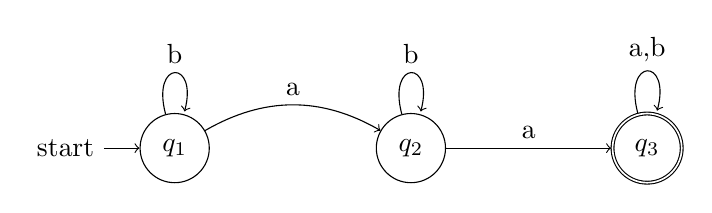
\begin{tikzpicture}[->, node distance = 3cm]
    \node[initial, state] (A) {$q_1$};
    \node[state](B) [right of = A] {$q_2$};
    \node[state, accepting] (C) [right of = B] {$q_3$};
    \path (A) edge [loop above] node{b} (A);
    \path (A) edge [bend left][above] node {a} (B);
    \path (B) edge [above] node {a} (C);
    \path (B) edge [loop above] node {b} (B);
    \path (C) edge [loop above] node {a,b} (C);
    \end{tikzpicture}
    \caption{Automaton}
\end{figure}
    
\end{frame}
\section{Blokcs}

% %BLOCK AND ALERT COMMANDS
\begin{frame}{Block 1}

In this slide, some important text will be
\alert{highlighted} because it's important.

\begin{block}{Remark}
Its a simple facebook group.
\end{block}

\begin{alertblock}{Important theorem}
Sample text in red box
\end{alertblock}

\begin{examples}
Sample text in green box. 
\end{examples}
\end{frame}
\section{Effects Demo}
% %EFFECTS DEMO
\setbeamercovered{transparent}
\begin{frame}{Effects Demo 1}
This is a sample line of text.

\begin{itemize}
 \item<1-> Text visible from slide 1 
 \item<2-> Text visible from slide 2
 \item<3> Text visible on slide 3
 \item<4-5> Text visible on slides 4 and 5
 \item<5-> Text visible from slide 5
 \item<6-> Text visible from slide 6
\end{itemize}
\end{frame}

% %EFFECTS DEMO USING PAUSE
\begin{frame}{Effects Demo 2}
 In this slide \pause

 the text will be partially visible \pause

 And finally everything will be there
\end{frame}
\section{Figure Section}
\begin{frame}{Adding Figure}
 \begin{figure}[h]
    \centering
    \includegraphics[scale = 0.5]{graph.png}
    \caption{Graph Theory}
    \label{fig:1}
\end{figure}   
\end{frame}
\section{Table Section}
\begin{frame}{Table}
\begin{tabular}{|c|c|c|c|}
    \hline
	1 & 2 & 3 & 4 \\ 
	\cline{1-3}
	1 & 2 & 3 & 4  \\
	\hline
	\multicolumn{3}{|c|}{text} & 4 \\
	\hline
	\multirow{2}{*}{text} & 2 & 3 & 4\\
	\cline{2-4}
	& 2 & 3 & 4 \\
	\hline
	\multicolumn{2}{|c|}{\multirow{2}{*}{text}} & \multicolumn{2}{|c|}{\multirow{2}{*}{anik}} \\
	\multicolumn{2}{|c|}{} & \multicolumn{2}{|c|}{} \\
	\hline
\end{tabular}
\end{frame}
\documentclass[28pt,a4paper]{article}
\usepackage[utf8]{inputenc}
\usepackage{lipsum}
\usepackage{color}
\usepackage{amsmath}
\usepackage{multirow}
\usepackage{multicol}
\usepackage{graphicx}
\usepackage{biblatex}
\usepackage{subfigure}
\usepackage{subcaption}
\usepackage{tikz}
\addbibresource{book.bib}
\title{CSE 300 - Class 1}
\author{Shehabul Islam Sawraz }
\date{\today}

\begin{document}
\maketitle

\section{Introduction}

\begin{figure}[h]
    

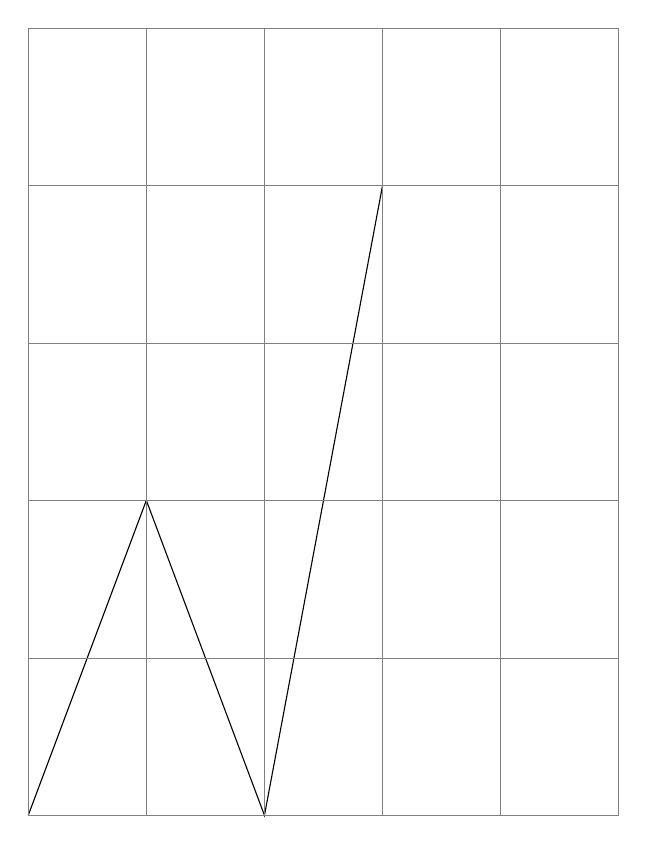
\begin{tikzpicture}[xscale=1.5, yscale=2]

\draw (0,0) -- (1,2) -- (2,0) -- (3,4);

\draw [help lines] (0,0) grid (5,5);

\end{tikzpicture}

\end{figure}

\begin{figure}[h]
    \centering
    \begin{tikzpicture}
    %\draw [|->] (-5,0) -- (5,0);
    %\draw [<->] (0,-5) -- (0,5); 

    %\draw [ultra thick] [<->] (0,5) -- (0,0) -- (5,0);

    %\draw [line width=8] [<->] (0,5) -- (0,0) -- (5,0);

    \draw [red][dotted, thick] [<->] (0,5) -- (0,0) -- (5,0);
    \end{tikzpicture}
    \caption{Caption}
    \label{fig:my_label}
\end{figure}

%Drawing a cure

\begin{tikzpicture}[h]

%\draw [blue] (0,0) rectangle (4,5);
%\draw [ultra thick] (0,0) circle [radius=3];
\draw (7,0) arc [radius=4,start angle=85, end angle=185];

\end{tikzpicture}
\label{fig:my_label}

\begin{tikzpicture}[h]

%\draw [blue] (0,0) rectangle (4,5);
%\draw [ultra thick] (0,0) circle [radius=3];
\draw [very thick] (0,0) to [out=90, in=125] (2,1.5);
\draw [help line] (0,0) grid (2,2);

\end{tikzpicture}
\label{fig:my_label}

\begin{tikzpicture}[h]

%\draw [blue] (0,0) rectangle (4,5);
%\draw [ultra thick] (0,0) circle [radius=3];
\draw [very thick] (0,0) to [out=90, in=180] (2,2) to [out=0, in=90] (4,0) to [out=-90, in=-180] (6,-2) to [out=0, in=-90] (8,0) to [out=90, in=180] (10,2) (10,2) to [out=0, in=90] (12,0) to [out=45, in=225] (14,2);
%\draw [very thick] (2,2) to [out=0, in=90] (4,0);
%\draw [very thick] (4,0) to [out=-90, in=-180] (6,-2);
%\draw [very thick] (6,-2) to [out=0, in=-90] (8,0);
%\draw [very thick] (8,0) to [out=90, in=180] (10,2);
%\draw [very thick] (10,2) to [out=0, in=90] (12,0);
%\draw [very thick] (12,0) to [out=45, in=225] (14,2);
\draw [help line] (0,0) grid (2,2);

\end{tikzpicture}

\begin{tikzpicture}

\draw [domain=0:1.5] plot (\x,{5+\x+\x*\x});

\end{tikzpicture}

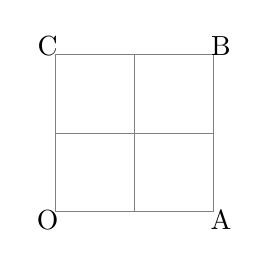
\begin{tikzpicture}

\draw [help lines] (0,0) grid (2,2);
\node at (-0.1,-0.1) {O};
\node at (2.1,-0.1) {A};
\node at (2.1,2.1) {B};
\node at (-0.1,2.1) {C};

\end{tikzpicture}

\begin{tikzpicture}

\draw [help lines] (0,0) grid (2,2);
\node [below left, green] at (0,0) {O};
\node [below right, red] at (2,0) {$A^x$};
\node [above right, yellow] at (2,2) {B};
\node [above left] at (0,2) {$C$};

\end{tikzpicture}



\end{document}
\begin{frame}{Drawing Grids and Axis}
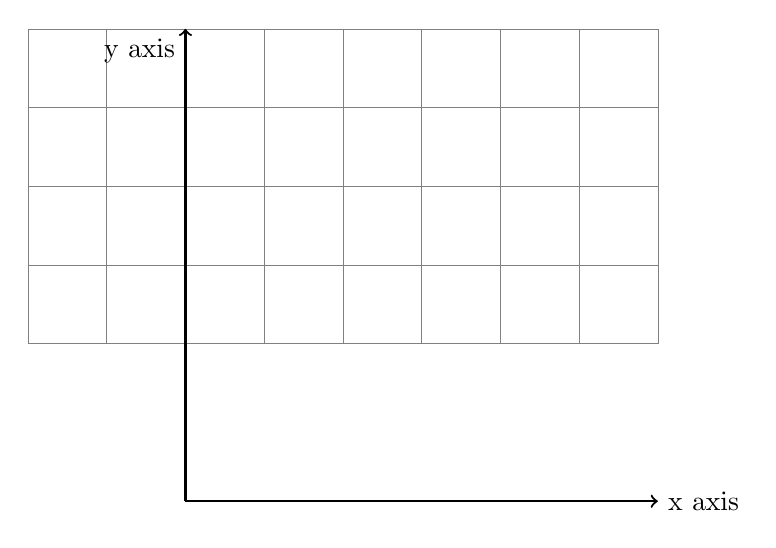
\begin{tikzpicture}
    \draw[step = 1cm, gray, very thin] (-2,2) grid (6,6);
    \draw[thick, ->](0,0)  -- (6,0) node[anchor = west] {x axis};
    \draw[thick, ->] (0,0) -- (0,6) node[anchor = north east] {y axis};
\end{tikzpicture}
    
\end{frame}
\section{Flow Chart}
\begin{frame}{Flow Chart}
    %For Flow Chart declaration
    \tikzstyle{startstop} = [ellipse, minimum width = 3cm, minimum height = 1cm, text centered, draw = black, fill = red!30]
    \tikzstyle{io} = [trapezium, trapezium left angle = 70, trapezium right angle = 110, minimum width = 3cm, minimum height = 1cm, text centered, draw = black, fill = blue!30]
    \tikzstyle{process} = [rectangle, minimum width = 3cm, minimum height = 1cm, text centered, draw = black, fill = orange!30]
    \tikzstyle{decision} = [diamond, aspect = 4, minimum width = 3cm, minimum height = 1cm, text centered, draw = black, fill = green!30 ]
    \tikzstyle{arrow} = [thick, ->, >=stealth]
    
    \begin{figure}
        \centering
        \begin{tikzpicture}
        \node[startstop] (start) {Start};
        \node[process, below of = start, yshift = -0.5cm] (p1) {Process - 1};
        \node[io, left of= p1, xshift = -3.5cm](io1) {Documents};
        \node[decision, below of = p1, yshift = -0.5cm] (d1) {Decision};
        \node[process, below of= d1, yshift = -0.5cm] (pA) {Process A};
        \node[process, below of= d1, yshift = -0.5cm, xshift = 3.5cm] (pB) {Process B};
        \node[startstop, below of = pA, yshift = -0.5cm] (end) {END};
        \draw[arrow] (start) -- (p1);
        \draw[arrow] (io1) -- (p1);
        \draw[arrow] (p1) -- (d1);
        \draw[arrow] (d1) -- node[right] {YES} (pA);
        \draw[arrow] (d1) -| node[above] {NO} (pB);
        \draw[arrow] (pA) -- (end);
        \draw[arrow] (pB) |- (end);
        
        \end{tikzpicture}
        \caption{Flow Chart}
        \label{fig:flow_chart}
    \end{figure}
\end{frame}
\section{Loop in Tikz}
\begin{frame}{Use of Loop in Tikz}
\begin{figure}
    \centering
    
\begin{tikzpicture}
    \foreach \x in {1,2,3,4}
    {\foreach \y in {1,2,3,4}
        {\draw (\x,\y) circle [radius=0.3];
        };
    }
    \end{tikzpicture}
    \caption{Use of Loop}
    \label{fig:loop}
\end{figure}
    
\end{frame}

\begin{frame}{Use of Loop in Tikz continue...}
\begin{figure}
    \centering
    \begin{tikzpicture}
    \draw[thick, ->](0,0)  -- (6,0) node[anchor = west] {x axis};
    \draw[thick, ->] (0,0) -- (0,6) node[anchor = north east] {y axis};
    \foreach \i\j\k in {1/A/0.5,2/B/1,3/C/1.5,4/D/2,5/E/2.5,6/F/3}
    {
        %\draw (0,0) circle [radius=\k];
        \node[draw,shape=circle] at (\i,2){\j};
        \pause
    }
 
    \end{tikzpicture}
    \caption{Fig 2}
\end{figure}
    
\end{frame}

\section{Complex Nodes}

\tikzstyle{place}=[circle,draw=blue!50,fill=blue!20,thick, inner sep=0pt,minimum size=6mm]
\tikzstyle{transition}=[rectangle,draw=black!50,fill=black!20,thick, inner sep=0pt,minimum size=4mm]


\begin{frame}{Complex Nodes}
\begin{figure}
    \centering
    \begin{tikzpicture}
\node[place] (waiting) {A};
\node[place] (critical) [below of=waiting] {B};
\node[place] (semaphore) [below of=critical] {C};
\node[transition] (leave critical) [right of=critical] {D}
edge [-> , bend right = 45] node[above] {1} (waiting);
\node[transition] (enter critical) [left of=critical] {E}
edge [->] node[above] {2} (critical)
edge [<-,bend left=45] (waiting)
edge [->,bend right=45] (semaphore);
\end{tikzpicture}
    \caption{Flow}
\end{figure}
\end{frame}



\begin{frame}{Complex Node 2}

\begin{figure}
    \centering
    \begin{tikzpicture}
\node[place] (waiting) {};
\node[place] (critical) [below of=waiting] {};
\node[place] (semaphore) [below of=critical] {};
\node[transition] (leave critical) [right of=critical] {};
\node[transition] (enter critical) [left of=critical] {};
\draw [->] (enter critical) -- (critical);
\draw [->] (waiting) to [in = 90, out = 180] node[anchor = south] {yoo} (enter critical);
\end{tikzpicture}
    \caption{Caption}
\end{figure}
    
\end{frame}
\section{Items}
\begin{frame}{Item Type 1}
This is an itemized list.
\begin{itemize}
    \item item 1
    \begin{itemize}
        \item nested item 1
        \item nested item 2
    \end{itemize}
    \item item 2
    \item item 3
\end{itemize}
\end{frame}

\begin{frame}{Item Type 2}
    This is an enumerated list.
\begin{enumerate}
    \item First item
    \item Second item
    \item This can also be nested.
    \begin{enumerate}
        \item nested item 1
        \item nested item 2
    \end{enumerate}
\end{enumerate}
\end{frame}

\begin{frame}{Item Type 3}

This is a descriptive list.
\begin{description}
\item[Number 1] one
\item[Number 2] two
\end{description}
    
\end{frame}

% \newpage

% \begin{frame}{Shape Drawing}
%  %draw rectangle
% \begin{tikzpicture}
% \draw[fill = blue!50, dashed] (0,0) rectangle (2,2) ; 
% \end{tikzpicture}

% %draw circle
% \begin{tikzpicture}
% \draw[red, thick] (2,2) circle (1);
% \draw (0,0) parabola (3,3);
% \end{tikzpicture}   
% \end{frame}


\end{document}
